\documentclass[12pt,letterpaper]{article}

\usepackage{fancyhdr}
\pagestyle{fancy}
\fancyhf{}
\rhead{Vaja 3}
\lhead{ORS}
\setlength{\headheight}{16pt}

\usepackage[utf8]{inputenc}
\usepackage[slovene]{babel}
\usepackage[colorlinks = true, urlcolor = blue]{hyperref}

\usepackage{xcolor}
\usepackage{listings}
\usepackage{graphicx}
\graphicspath{{./images/}}
\definecolor{mGreen}{rgb}{0,0.6,0}
\definecolor{mGray}{rgb}{0.5,0.5,0.5}
\definecolor{mPurple}{rgb}{0.58,0,0.82}
\definecolor{backgroundColour}{rgb}{1,1,1}

\lstdefinestyle{CStyle}{
    backgroundcolor=\color{backgroundColour},   
    commentstyle=\color{mGreen},
    keywordstyle=\color{magenta},
    numberstyle=\tiny\color{mGray},
    stringstyle=\color{mPurple},
    basicstyle=\footnotesize,
    breakatwhitespace=false,         
    breaklines=true,                 
    captionpos=b,                    
    keepspaces=true,                 
    numbers=left,                    
    numbersep=5pt,                  
    showspaces=false,                
    showstringspaces=false,
    showtabs=false,                  
    tabsize=2,
    language=C,
    frame=none
}

\begin{document}

\begin{center}
    \textbf{\Large Izdelava knjižnice za delo s splošno namenskim vhodom/izhodom}   
\end{center}

Na razvojni plošči STM32F4Discovery, ki jo uporabljamo na vajah, je vgrajen mikrokrmilnik STM32F407, le-ta ima 140 pinov, ki jih lahko uporabimo kot digitalni vhod, digitalni izhod ali pa prepustimo da s pini upravljajo druge naprave znotraj mikrokrmilnika. Gre torej za splošnonamenski pine (angl. General Purpose Input Output), ki jih običajno označujemo s kratico GPIO.

V mikrokrmilniku STM32F407 so pini razdeljeni v 9 GPIO naprav (angl. GPIO Port) s črkovnimi oznakami od A do I. Naprave A do H imajo vsaka po 16 pinov, naprava I pa upravlja s preostalimi dvanajstimi. Pini znotraj naprav so označeni s števili od 0 do 15. Posamezne pine mikrokrmilnika tako označujemo s črko P, sledi črka naprave ter številka pina znotraj naprave. Na primer PA0 (pin 0 na napravi A) ali PD12 (pin 12 na napravi D). Takšne oznake lahko vidite tudi na sami razvojni plošči (glej sliko \ref{smt32f4discovery}).

\begin{figure}[ht!]
  \centering
  \caption{STM32F4 Discovery.}
  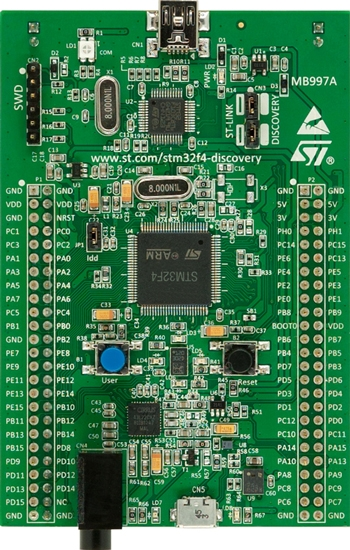
\includegraphics[height=180pt]{images/vaja3/stm32f4_discovery.jpg}
  \label{smt32f4discovery}
\end{figure}

Vse naprave imajo vnaprej dodeljen pomnilniški prostor. Primer dodeljenih prostorov je prikazan na sliki \ref{naslovi}. V tem pomnilniškem prostoru se nahajajo registri naprav. Ti hranijo vse nastavitve naprave, prav tako pa preko njih beremo stanje naprave oziroma jo upravljamo.

\begin{figure}[ht!]
  \centering
  \caption{Naslovi naprav.}
  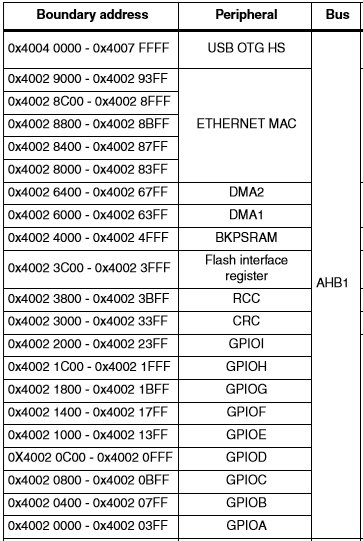
\includegraphics[height=190pt]{images/vaja3/naslovi.png}
  \label{naslovi}
\end{figure}


\section*{Vklop ure GPIO naprave}

Če želimo uporabiti posamezen GPIO pin, moramo najprej vklopiti napravo, ki ji pin pripada. Za vklop ure skrbi naprava \texttt{Reset and Clock Control (RCC)}. Vklopu ur GPIO naprav je namenjen register \texttt{RCC\_AHB1ENR}. Slika \ref{ahb1enr} prikazuje izsek dokumentacije mikrokrmilnika o tem registru. Kot vidimo, gre za 32-bitni register, kjer je spodnjih devet bitov namenjenih vklopu in izklopu ure GPIO naprav. Bit 0 ima oznako \texttt{GPIOAEN} in skrbi za vklop ure naprave A, bit 1 skrbi za uro naprave B, in tako dalje vse do bita 8, ki skrbi za vklop in izklop ure naprave GPIOI. Edino vprašanje, ki se nam tukaj še poraja je, na katerem naslovu se ta register nahaja. V izseku dokumentacije, ki ga prikazuje slika \ref{ahb1enr} je namreč podan zgolj odmik naslova znotraj naprave (angl. Address offset).

Kot vidimo na sliki \ref{ahb1enr} je ta odmik pri registru \texttt{RCC\_AHB1ENR} 0x30. Dejanski naslov dobimo tako, da odmik prištejemo začetnemu naslovu naprave RCC. Tega lahko najdete na sliki \ref{naslovi}. Za napravo RCC je zapisan začetni naslov 0x40023800. Točen naslov registra \texttt{RCC\_AHB1ENR} je torej 0x40023830. Če preverite rešitve vaših nalog iz pretekle vaje, boste opazili, da ste za vklop ure na tem naslovu postavljali bita 0 in 3. S tem se vklopili uri za napravi GPIOA in GPIOD (gumb integriran na plošči se nahaja na PA0, led diode pa na PD12, PD13, PD14 in PD15).

\begin{figure}[ht!]
  \centering
  \caption{Register AHB1ENR naprave RCC.}
  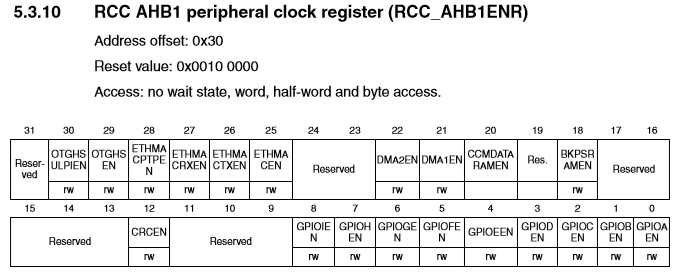
\includegraphics[height=140pt]{images/vaja3/ahb1enr.png}
  \label{ahb1enr}
\end{figure}


\section*{Inicializacija GPIO naprave}

Po vklopu ure lahko določamo nastavitve posameznih pinov. Za vsakega izmed šestnajstih pinov ima GPIO naprava enako vhodno/izhodno stopnjo, ki je prikazana na sliki \ref{vhodno_izhodna_stopnja}. Zgornji del prikazuje vhodni del, spodnji pa izhodnega. Obema deloma je skupna zgolj uporaba zaščitnih diod (angl. Protection diode) ter Pull-up in Pull-down uporov. Uporaba slednjih je opcijska in jo lahko nastavimo tako za vhodne kot izhodne pine. V primeru, da pin uporabimo kot vhod, je to tudi (poleg nastavitve da gre za vhodni pin) edina nastavitev, ki jo je potrebno določiti. Logično stanje na vhodu nato beremo preko registra \texttt{Input Data (IDR)}.
V primeru, da pin deluje kot izhod, je potrebno nastaviti še način izhoda (Push-pull ali open-drain) ter hitrost osveževanja vrednosti na izhodu. Po izbiri teh nastavitev stanje na izhodu določamo preko registra \texttt{Output Data (ODR)} ali preko registrov \texttt{Bit set/reset (BSRR)}.

\begin{figure}[ht!]
  \centering
  \caption{Vhodno/izhodna stopnja.}
  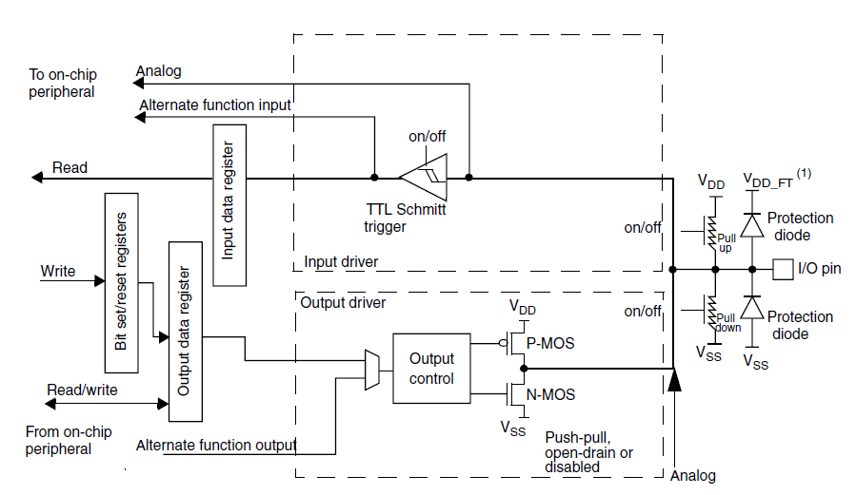
\includegraphics[height=200pt]{images/vaja3/vhodno_izhodna_stopnja.png}
  \label{vhodno_izhodna_stopnja}
\end{figure}

Način delovanja (angl. mode) pina določimo v registru \texttt{Mode (MODER)}. Slika \ref{moder} prikazuje izsek dokumentacije, ki opisuje omenjeni register. Kot vidimo na sliki, gre za 32-bitni register, ki je razdeljen v šestnajst dvo-bitnih delov, vsak namenjen enemu pinu. Bita 0 in 1 tako služita za nastavljanje načina delovanja pina 0 izbrane naprave, bita 2 in 3 nastavljata način delovanja pina 1, bita 4 in 5 pina 2 in tako dalje do bitov 30 in 31, ki nastavljata način delovanja pina 15. Na sliki je ravno tako prikazano, da nastavitev bitov na vrednost 00 (oba bita 0) pomeni, da pin deluje kot vhod, vrednost 01 (zgornji bit 0, spodnji bit 1) pa pomeni izhod. Preostali vrednosti določita analogni način delovanja (10) in način alternativne funkcije (11), ki pomeni, da s pinom upravlja ena izmed preostalih naprav mikrokrmilnika. Slednja dva načina bomo podrobneje spoznali na vajah v nadaljevanju semestra. Kot vidimo, je odmik naslova 0x00, kar pomeni, da se ta register vedno nahaja na začetku pomnilniškega prostora posamezne naprave. Za napravo A torej na naslovu 0x40020000 in za napravo D na naslovu 0x40020C00. Na prvi naslov ste v zadnji vaji morali na bita 0 in 1 vpisati ničli. S tem ste določili, da bo v napravi A pin 0 deloval kot vhod (na tem pinu najdemo integriran gumb). Na drugi naslov pa ste na zgornjih osem bitov zapisali vrednost 01. Kar pomeni, da ste pine 12, 13, 14 in 15 naprave D nastavili v izhodni način delovanja (na teh štirih pinih najdemo integrirane led diode).

\begin{figure}[ht!]
  \centering
  \caption{Register MODE naprave GPIO.}
  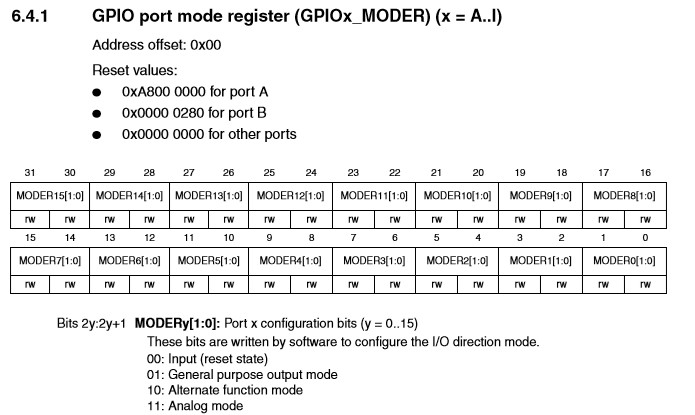
\includegraphics[width=350pt]{images/vaja3/moder.png}
  \label{moder}
\end{figure}

Če želimo pin uporabiti kot vhod, je edina nastavitev, ki jo še moramo nastaviti, uporaba pull-up in pull-down uporov. Pull-up ali pull-down upore najpogosteje uporabljamo, da preprečimo ``plavanje'' (angl. float) na vhodnih ali izhodnih pinih. V primeru da na pinu ni drugih virov, s pull-up uporom lahko dosežemo, da je na pinu logična enica, medtem ko s pull-downom uporom dosežemo, da je takrat na pinu logična ničla. Ti upori imajo še več drugih primerov uporabe, v katere pa se zaenkrat ne bomo podrobno spuščali. Zaenkrat bomo za vse pine, ki jih bomo uporabljali, nastavljali, da ne uporabljajo omenjenih uporov. To nastavitev določimo v registru \texttt{Pull-up, Pull-down (PUPDR)}. Izsek iz dokumentacije je prikazan na sliki \ref{pupdr}.

\begin{figure}[ht!]
  \centering
  \caption{Register PUPD naprave GPIO.}
  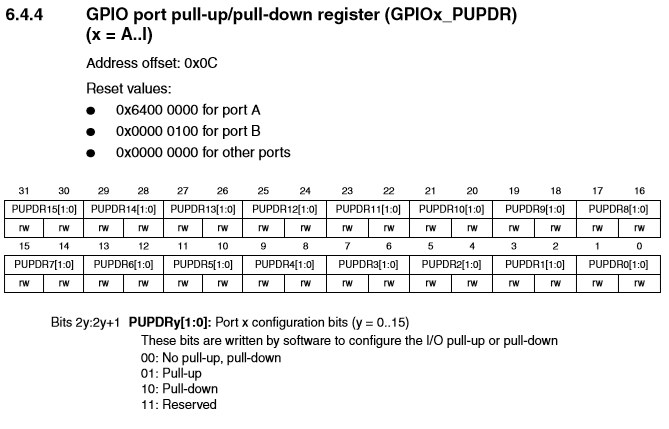
\includegraphics[width=350pt]{images/vaja3/pupdr.png}
  \label{pupdr}
\end{figure}

Podobno kot register \texttt{MODER}, je tudi \texttt{PUPDR} 32-bitni register, kjer sta po dva bita sta namenjana posameznemu pinu. Vpisana vrednost 00 pomeni, da na pinu ne želimo uporabiti niti pull-up niti pull-down upora. Z vpisom 01 vklopimo pull-up, z vpisom 10 pa pull-down. Vrednost 11 je rezervirana (prepovedana) in se je ne uporablja. Odmik naslova registra \texttt{PUPDR} je 0x0C.

Če želimo pin uporabiti kot izhod moramo poleg zgoraj omenjenih registrov nastaviti še registra, ki določata način izhoda ter hitrost osveževanja. Hitrost osveževanja določamo v registru \texttt{Output Speed (OSPEEDR)}, ki je prikazan na sliki \ref{ospeedr}. Po strukturi je register podoben prej opisanima registroma. V primeru registra \texttt{OSPEEDR} vpis vrednosti 00 pomeni, da bo hitrost osveževanja 2MHz, vpis vrednosti 01 pomeni, da bo hitrost osveževanja 25 MHz, preostali kombinaciji (10 in 11) pa nastavita hitrost osveževanja na 50 ali 100 MHz. Odmik naslova registra \texttt{OSPEEDR} je 0x08. Za vse pine, ki jih bomo uporabljali pri predmetu ORS, bo zadostovala najnižja hitrost osveževanja.

\begin{figure}[ht!]
  \centering
  \caption{Register OSPEEDR naprave GPIO.}
  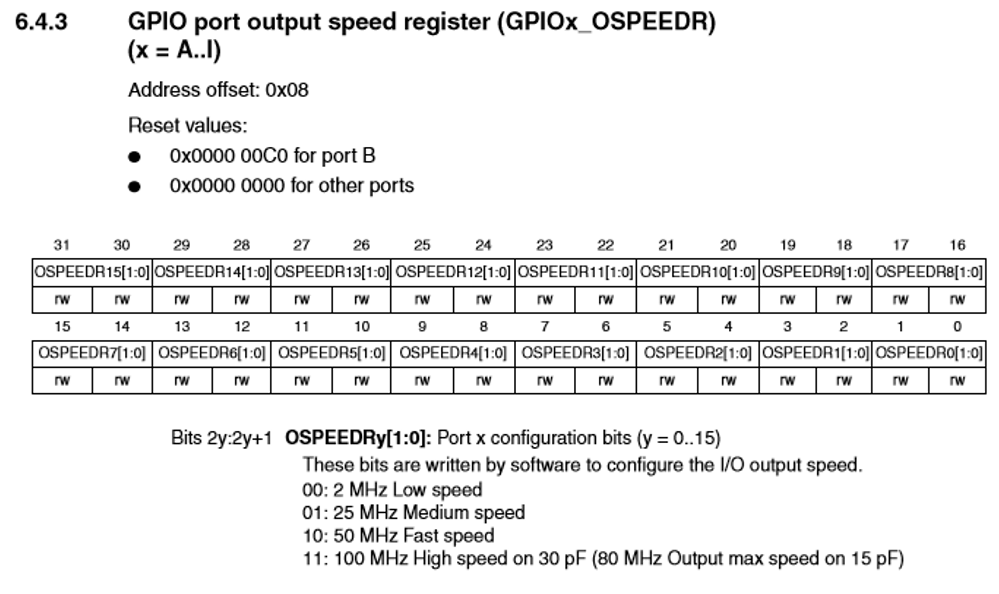
\includegraphics[width=350pt]{images/vaja3/odpspeedr.png}
  \label{ospeedr}
\end{figure}

Preostane nam še register v katerem določimo način izhoda. Načina izhoda sta push-pull in open-drain. Več o razliki med njima boste spoznali na predavanjih. Če na povzamemo na kratko, se pri push-pull pri ničli izhod vleče (angl. pull) proti ozemljitvi (GND, angl. ground) in potiska proti viru napajanja (VDD) pri enici. Pri open-drain pa se izhod pri ničli obnaša podobno, pri logični enici pa je izhod v visoki impendanci. V navezavi z open-drain načinom izhoda se zato običajno uporablja pull-up upor. Na vajah bo način izhoda vedno push-pull, razen če bomo izrecno poudarili. Za LED diode tako izhod vedno nastavimo na push-pull. Register, ki nastavlja način izhoda se imenuje \texttt{Output Type (OTYPER)}. V dokumentaciji (slika \ref{otyper}) vidimo, da je tudi ta register 32-bitni, vendar pa se dejansko uporablja zgolj spodnjih 16 bitov. Vsak bit nastavlja način izhoda za en pin. Bit 0 za pin 0, bit 1 za pin 1, in tako dalje do bita 15, ki nastavlja način izhoda za pin 15. Odmik naslova tega registra je 0x04.

\begin{figure}[ht!]
  \centering
  \caption{Register OTYPER naprave GPIO.}
  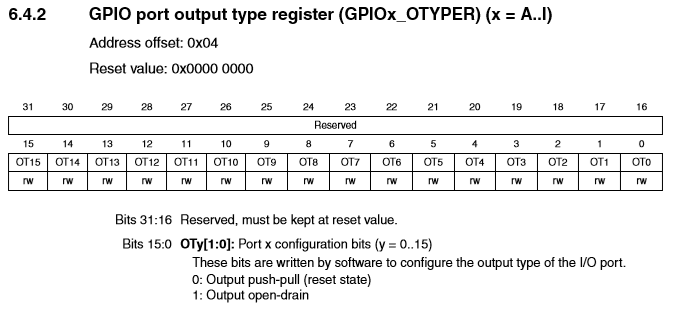
\includegraphics[width=350pt]{images/vaja3/otyper.png}
  \label{otyper}
\end{figure}


\section*{Branje vhoda GPIO naprave}

Za branje vhoda uporabljamo register \texttt{Input Data (IDR)}, ki je prikazan tudi na sliki \ref{vhodno_izhodna_stopnja}. Ta register se znotraj registrov naprave nahaja na odmiku 0x10. Kot prikazuje dokumentacija na sliki \ref{idr}, je tudi ta register 32-bitni, vendar je podobno kot pri \texttt{OTYPER} uporabljenih zgolj spodnjih 16 bitov.

\begin{figure}[ht!]
  \centering
  \caption{Register IDR naprave GPIO.}
  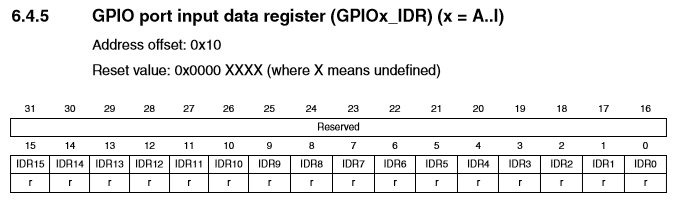
\includegraphics[width=350pt]{images/vaja3/idr.png}
  \label{idr}
\end{figure}

Za razliko od registrov, ki smo jih do sedaj spoznali, se bite tega registra da samo brati (angl. read-only). To je označeno s črko \textit{r} pod oznakami bitov. Posamezen bit predstavlja logično vrednost na vhodu. Če je na vhodnem pinu visoka napetost, potem bo na bitu, ki predstavlja stanje pina, enica. Če je na vhodnem pinu nizka napetost, potem bo na bitu, ki predstavlja stanje pina, ničla. Ker je gumb, ki ste ga uporabljali na zadnji vaji, vezan na pin PA0, ste stanje gumba brali tako, da ste preverjali stanje bita 0 na naslovu 0x40020010 (0x4002000 zaradi naprave A + 0x10 zaradi odmika registra).


\section*{Nastavljanje izhoda GPIO naprave}

Za nastavljanje vrednosti na izhodu imamo dve možnosti. Neposredno nastavljanje registra \texttt{Output Data (ODR)} ali pa posredno nastavljanje preko para set/reset registrov. Register ODR (slika \ref{odr}) se znotraj registrov naprave nahaja na odmiku 0x14. Podobno kot pri registru \texttt{IDR} tu uporabljamo zgolj spodnjih 16-bitov, le da tu mi nastavljamo posamezne bite na 0 ali 1 in s tem neposredno spreminjamo napetost na istoležnih izhodnih pinih. Primer: vpis enice na bit 5 pomeni, da bo na pinu 5 te naprave visoka napetost. Vpis ničle na isti bit pa povzroči, da je na pinu 5 nizka napetost. Oboje se zgodi le v primeru, da je pin v izhodnem načinu delovanja.

\begin{figure}[ht!]
  \centering
  \caption{Register ODR naprave GPIO.}
  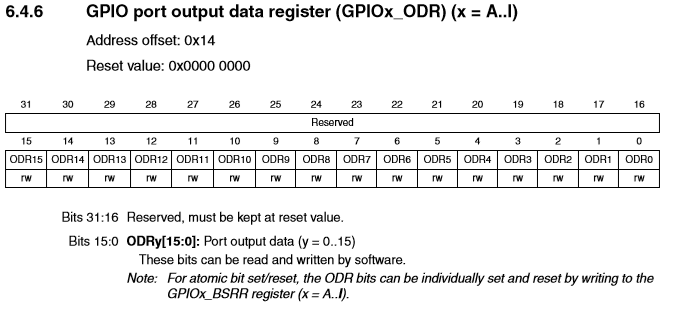
\includegraphics[width=350pt]{images/vaja3/odr.png}
  \label{odr}
\end{figure}

Če želimo spremeniti vrednost določenega bita v registru \texttt{ODR}, moramo vrednost registra ODR najprej prebrati, nato z logično operacijo in/ali spremeniti njegovo vrednost ter vrednost zapisati nazaj na naslov. Kot smo spoznali na prvih vajah, bi programsko postavljanje p-tega bita zapisali kot \texttt{ODR = ODR | (1 << p)}, brisanje pa kot \texttt{ODR = ODR \& \~(1 << p)}. Vsaka izmed teh operacij potrebuje tri korake za izvedbo: branje vrednosti, izračun ter pisanje vrednosti (angl. read-modify-write).

Mikrokrmilnik STM32F407 omogoča, da obe operaciji izvedemo bolj učinkovito, in sicer preko registrov set in reset. Izsek iz dokumentacije teh dveh registrov je prikazan na sliki \ref{bsrr}. Na sliki sta prikazan kot en register, dejansko pa gre za dva 16-bitna registra. Oba registra omogočata zgolj vpis (angl. write-only). In sicer vpis enice na bit $p$ registra \texttt{Bit Set (BSR)} pomeni, da se na bit $p$ v registru \texttt{ODR} vpiše enica. Vpis \textbf{enice} na bit $p$ registra \texttt{Bit Reset (BRR)} pa pomeni, da se na bit $p$ v registru \texttt{ODR} vpiše \textbf{ničla}. Ko se sprememba vrednosti v registru \texttt{ODR} izvede, se registra \texttt{BSR} in \texttt{BRR} ustrezno počistita. Register \texttt{BSR} se nahaja na odmiku 0x18, register \texttt{BRR} pa na odmiku 0x1A. Na zadnji vaji ste LED diode prižigali z vpisovanjem enic na naslov 0x40020C18, ugašali pa z vpisovanjem enic na naslov 0x40020C1A. Prva vrednost predstavlja naslov \texttt{BSR} registra naprave GPIOD, druga pa naslov \texttt{BRR} registra iste naprave.

\begin{figure}[ht!]
  \centering
  \caption{Register BSRR naprave GPIO.}
  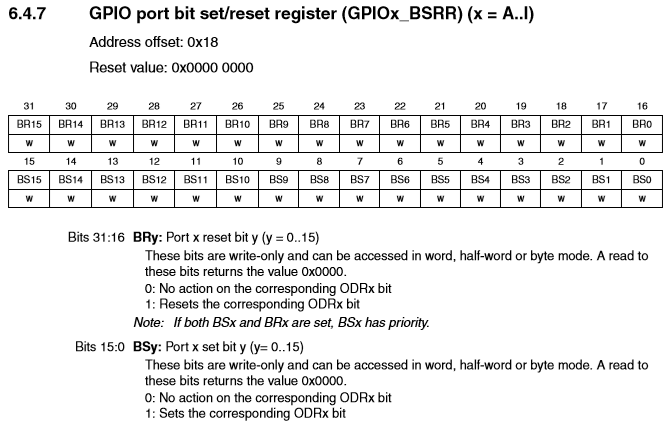
\includegraphics[width=350pt]{images/vaja3/bsrr.png}
  \label{bsrr}
\end{figure}

Registri GPIO naprave, ki smo jih pravkar spoznali, si v pomnilniškem prostoru ene naprave sledijo tako kot prikazuje tabela \ref{nasloviRegistrov}.

\begin{table}[ht!]
    \caption{Odmiki registrov GPIO naprave.}
    \centering
        \begin{tabular}{|l|l|}
            \hline
            Odmik naslova & Register                  \\ \hline
            0x00          & Mode (MODER)              \\ \hline
            0x04          & Output Type (OTYPER)      \\ \hline
            0x08          & Output Speed (OSPEEDR)    \\ \hline
            0x0C          & Pull-up/Pull-down (PUPDR) \\ \hline
            0x10          & Input Data (IDR)          \\ \hline
            0x14          & Output Data (ODR          \\ \hline
            0x18          & Bit Set (BSR)             \\ \hline
            0x1A          & Bit Reset (BRR)           \\ \hline
        \end{tabular}
    \label{nasloviRegistrov}
\end{table}

\subsection*{Funkcije pinov}

Kot smo že zapisali, se gumb na razvojni plošči STM32F4 Discovery nahaja na pinu PA0, medtem ko so štiri LED diode povezane na pine PD12, PD13, PD14 in PD15. Verjetno se sprašujete, kako bi ta isti podatek lahko izbrskali sami. Podatki o tem kam so povezani posamezni na razvojni plošči so zapisani v uporabniškem priročniku (angl. User manual), ki ga najdete na učilnici ali na spletni strani proizvajalca (\href{https://www.st.com/content/ccc/resource/technical/document/user_manual/70/fe/4a/3f/e7/e1/4f/7d/DM00039084.pdf/files/DM00039084.pdf/jcr:content/translations/en.DM00039084.pdf}{povezava}). V priročniku lahko na straneh od 20 do 28 najdete tabelo, katere izsek je prikazan na sliki \ref{usermanualpini}. Na sliki vidimo potrditev, da je zelena LED dioda vezana na pin PD12, oranžna na PD13, rdeča na PD14 ter modra na PD15. Prav tako na desni strani vidite, da je uporabniški (angl. User) gumb vezan na pin PA0.

\begin{figure}[ht!]
  \centering
  \caption{Izsek iz uporabniškega priročnika.}
  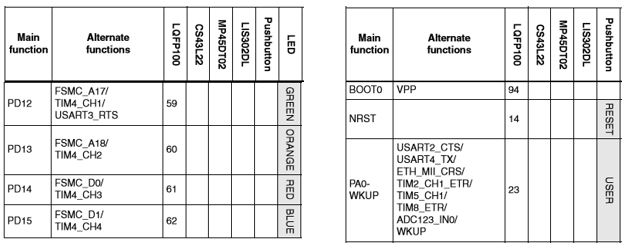
\includegraphics[width=350pt]{images/vaja3/usermanualpins.JPG}
  \label{usermanualpini}
\end{figure}

\subsection*{Uporaba konstant in struktur za delo s specifičnimi naslovi}

Z načinom pisanja kode za delo z GPIO, kot smo jo pisali na prejšnji vaji, bi težko naredili kak večji projekt. Kot vas je večina ugotovila, je takšno kodo, ki vsebuje polno neposredno vpisanih naslovov in konstant, težko brati in razhroščevati. Najmanj, kar bi lahko naredili je, da vsem konstantam in naslovom dajemo opisna imena in jih zberemo na enem mestu (na vrhu datoteke ali v ločeni .h datoteki), saj jih bo tako lažje preverjati in vzdrževati.

Za primer vzemimo Bit Set (\texttt{BSR}) register naprave GPIOD, ki se nahaja na naslovu 0x40020C18. Namesto, da v funkcijah uporabljamo direktno vrednost naslova, lahko temu naslovu dodelimo neko ime, ki nam pove kaj ta naslov predstavlja (na primer \texttt{GPIOD\_BIT\_SET\_REG}). Prav tako lahko dodelimo smiselna imena konstantam, ki jih uporabljamo za delo z registrom. Primer takih konstant lahko vidite spodaj:

\begin{center}
\begin{lstlisting}[style=CStyle]
    #define GPIOD_BIT_SET_REG 0x40020C18
    #define PIN_0 0x0001
    #define PIN_1 0x0002
    #define PIN_2 0x0004
    #define PIN_3 0x0008
\end{lstlisting}
\end{center}

S takšnimi konstantami bi vklop pinov zapisali kot

\begin{center}
\begin{lstlisting}[style=CStyle]
    uint32_t *p = (uint32_t *) GPIOD_BIT_SET_REG;
    *p = PIN_0;
    // vklopimo lahko tudi vec pinov hkrati
    *p = PIN_1 | PIN_2;
\end{lstlisting}
\end{center}

Zgornjo uporabo lahko še dodatno optimiziramo tako, da konstanto, ki predstavlja naslov registra, spremenimo v kazalec. S tem se izognemo prvi vrstici v zgornjemu primeru.

\begin{center}
\begin{lstlisting}[style=CStyle]
    #define GPIOD_BIT_SET_REG ((uint16_t*)0x40020C18)
    #define PIN_0 0x0001
    #define PIN_1 0x0002
    #define PIN_2 0x0004
    #define PIN_3 0x0008
    
    *GPIOD_BIT_SET_REG = PIN_0;
    *GPIOD_BIT_SET_REG = PIN_1 | PIN_2;
\end{lstlisting}
\end{center}

Kot smo videli na primeru GPIO naprav, imajo vse naprave mikrokrmnilnika množico registrov, ki jih moramo nastavljati, ko te naprave uporabljamo. Registri posamezne naprave se vedno nahajajo na zaporednih naslovih v pomnilniku. Z uporabo zgornjega pristopa bi 4 zaporedne registre ene naprave lahko nastavili na sledeč način:

\begin{center}
\begin{lstlisting}[style=CStyle]
    #define NAPRAVA_REG1	((uint32_t *) 0x40020C00)
    #define NAPRAVA_REG2	((uint16_t *) 0x40020C04)
    #define NAPRAVA_REG3	((uint16_t *) 0x40020C06)
    #define NAPRAVA_REG4	((uint32_t *) 0x40020C08)
    
    // registrom dolocimo vrednosti
    *NAPRAVA_REG1 = 0x8000;
    *NAPRAVA_REG2 = 0x4000;
    *NAPRAVA_REG3 = 0x6000;
    *NAPRAVA_REG4 = 0x5000;
\end{lstlisting}
\end{center}

Z uporabo strukture, ki opisuje registre naprave lahko omenjeno kodo še dodatno izbojšamo. Vemo namreč, da se vsi elementi strukture nahajajo na zaporednih naslovih. S tem se izognemu ponavljanju celotnih naslovov za vsak register posebej. Navedemo namreč zgolj začetni naslov naprave. Če je struktura pravilno sestavljena (predstavlja pomnilniško sliko naprave) bodo potem vsi elementi strukture kazali na pravilne registre.

\begin{center}
\begin{lstlisting}[style=CStyle]
    struct naprava_x {
    	uint32_t REG1;
    	uint16_t REG2;
    	uint16_t REG3;
    	uint32_t REG4;
    };
    
    #define	NAPRAVA 0x40020C00
    
    struct naprava_x * x;
    x = (struct naprava_x *) NAPRAVA;
    
    // registrom dolocimo vrednosti
    x->REG1 = 0x8000;
    x->REG2 = 0x6000;
    x->REG3 = 0x4000;
    x->REG4 = 0x5000;
\end{lstlisting}
\end{center}

Če zopet uporabimo trik, da je konstanta kazalec, lahko kodo naredimo bolj berljivo ter jo še dodatno skrajšamo:

\begin{center}
\begin{lstlisting}[style=CStyle]
    struct naprava_x {
    	uint32_t REG1;
    	uint16_t REG2;
    	uint16_t REG3;
    	uint32_t REG4;
    };
    
    #define	NAPRAVA ((struct naprava_x *) 0x40020C00)
    
    // registrom dolocimo vrednosti
    NAPRAVA->REG1 = 0x8000;
    NAPRAVA->REG2 = 0x6000;
    NAPRAVA->REG3 = 0x4000;
    NAPRAVA->REG4 = 0x5000;
\end{lstlisting}
\end{center}

Omenjen zapis morda res ni krajši kot tisti, iz katerega smo začeli, a se je bistveno zmanjšalo število fiksno zapisanih naslovov v naši kodi. To pa posledično pomeni bistveno manjšo možnost za vnos napak. Če upoštevamo še dejstvo, da lahko zapisano strukturo uporabimo na več mestih (isto strukturo za GPIO lahko uporabimo za vseh devet GPIO naprav) pa smo s tem zapisom tudi močno skrajšali našo kodo.


\section*{Naloga}

Iz učilnice naložite izhodiščno main.c datoteko za vaš projekt. Rešite naslednje naloge::

\begin{itemize}
    \item Sestavite strukturo, ki predstavlja GPIO napravo. Elementi strukture naj imajo smiselna imena iz katerih se enostavno razbere njihov pomen.
    \item Napišite funckijo \texttt{clock\_on}, ki vklopi uro podane naprave. Primera uporabe: \texttt{clock\_on(GPIOAd); clock\_on(GPIOCd)};
    \item Napišite funckijo \texttt{init\_GPIO}, ki izbran pin nastavi na poljubne nastavitve. Primera uporabe:
    \newline \texttt{init\_GPIO(GPIODd, 12, OUT, NO\_PULL, PUSH\_PULL, S2MHz);}
    \newline \texttt{init\_GPIO(GPIOAd, 0, IN, NO\_PULL, PUSH\_PULL, S2MHz);}
    \newline Prvi argument funckije je naprava, ki ji pin pripada (od \texttt{GPIOAd} do \texttt{GPIOId}), drugi argument je številka pina, sledijo način delovanja (\texttt{IN}, \texttt{OUT}, \texttt{AF} ali \texttt{ANALOG}), kjer kratica \texttt{AF} predstavlja alternativno funkcijo, uporaba pull-up/pull-down uporov (\texttt{NO\_PULL}, \texttt{PULL\_UP} ali \texttt{PULL\_DOWN}), način izhoda (\texttt{PUSH\_PULL} ali \texttt{OPEN\_DRAIN}) ter na koncu hitrost osve\-že\-va\-nja (\texttt{S2MHz}, \texttt{S25MHz}, \texttt{S50MHz} ali \texttt{S100MHz}).
    \item Napišite funkcijo za vklop/izklop izhodnega pina, ki nastavi izbrani pin na podano vrednost: \texttt{GPIO\_pin\_write(naprava, pin, vrednost)}.
    \item Napišite funkcijo za branje stanja vhodnega pina, ki vrne enico, če je stanje podanega pin na vhodu ena oziroma ničlo, če je stanje podanega pina ničla: \texttt{GPIO\_pin\_read(naprava, pin)}.
    \item Uporabite spisane funkcije za proženje led sekvence ob pritisku na gumb, led sekvenca naj bo enaka kot pri prejnji vaji. Torej ob pritisku na uporabniški gumb (gumb modre barve), naj se najprej z zamikom prižge vsaka ledica posebej, ko so vse led diode prižgane, se po kratkem zamiku ugasnejo.
\end{itemize}

\subsection*{Pomoč in namigi}

\begin{itemize}
    \item Gumb se nahaja na pinu PA0. Pin nastavite kot vhod brez pull-up ali pull-down uporov.
    \item LED diode se nahajajo na pinih PD12, PD13, PD14, PD15. Vse pine LED diod inicializirajte kot izhod, brez pull-up ali pull-down uporov in z načinom izhoda push-pull. Hitrost osveževanja lahko nastavite na najnižjo.
\end{itemize}

\end{document}
